A single film does not have the necessary interactions to fulfill the neutron count rate criteria multiple films are necessary, and the arrangement of these films provides a design space for a replacement RPM.
In the case of the RPM, there are several design parameters that can be explored:
\begin{itemize}
  \item the neutron absorber loading of the film,
  \item the thickness of the film,
  \item the geometry of the film (cylinders or sheets), and
  \item the placement of the films.
\end{itemize}
It is expected that the loading of the film will be limited by the optical clarity, and that the thickness of the film will be determined by the optimization of the energy deposition.
Thus, of the above design parameters only the geometric placement of the films is an available optimization space.

Preliminary work by this author provided a simple design in which the detector layers are linearly placed throughout the detector volume in an alternating fashion.
The analysis of the neutron flux throughout this detector lead to a flat flux profile as shown in \autoref{fig:AltLayerThermalNeutronFraction}.
\begin{figure}
  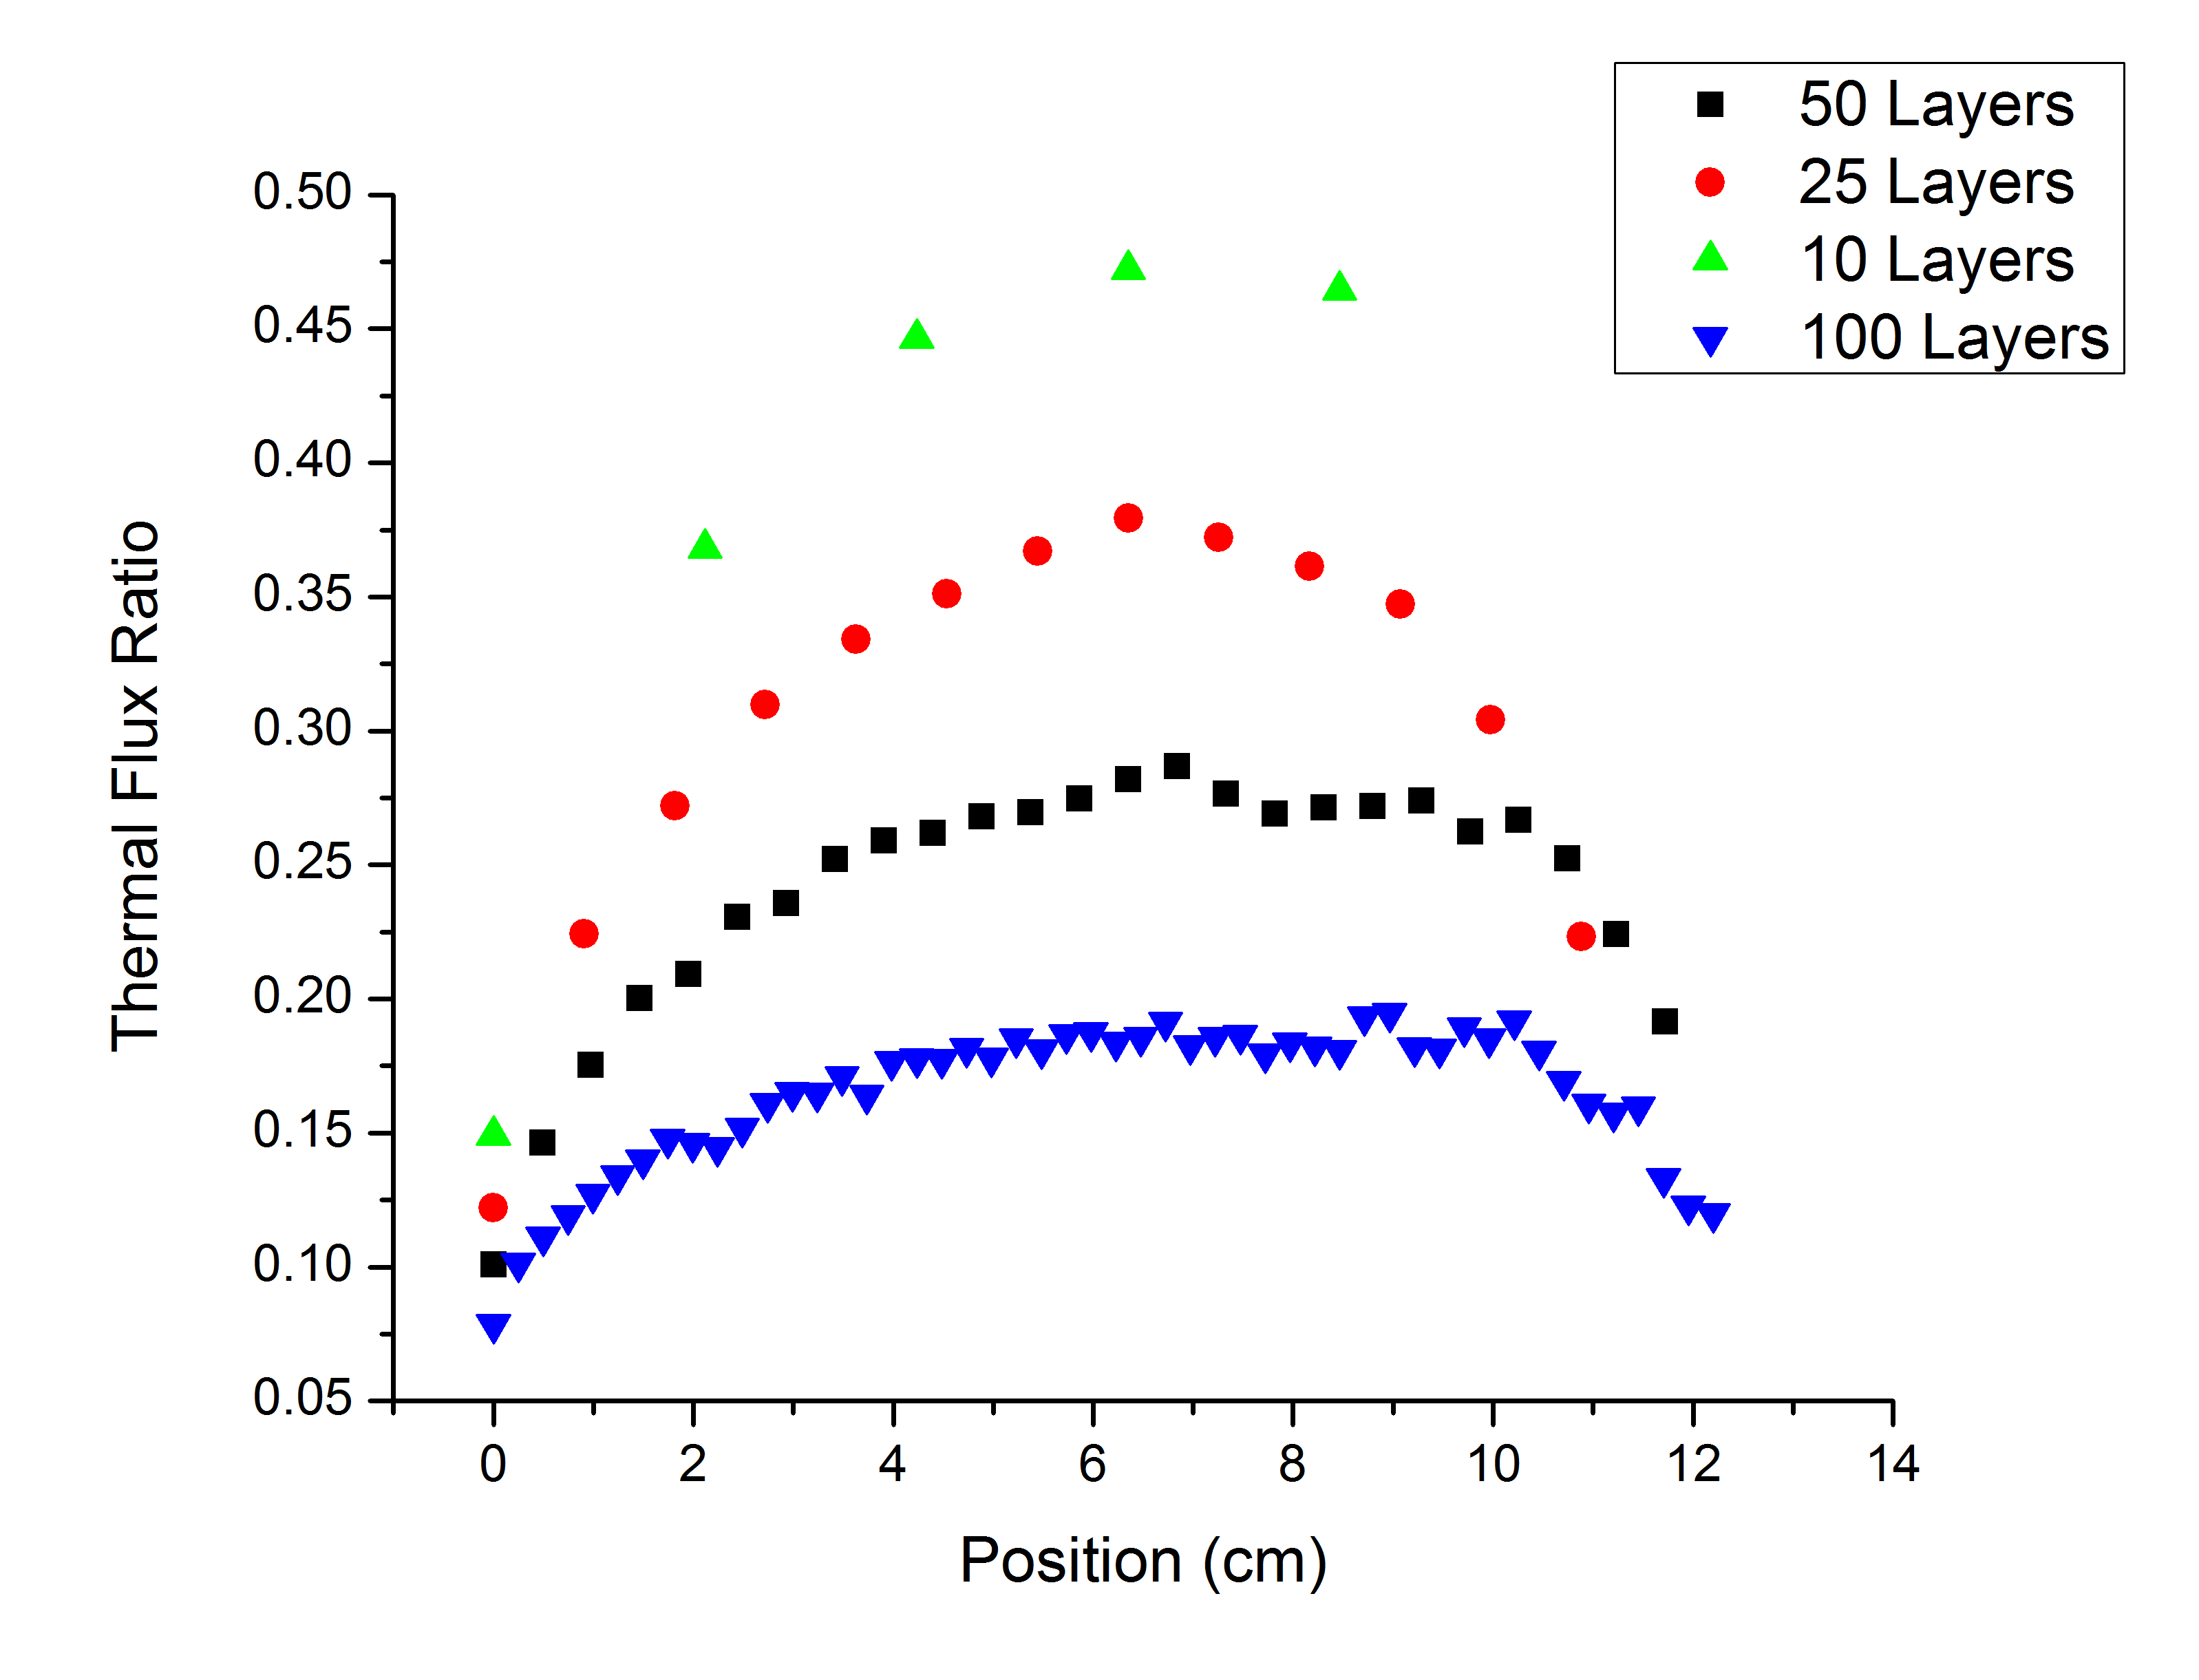
\includegraphics[width=\textwidth]{ThermalFluxRatioAltLayers}
	\caption{Fraction of the neutron flux that is thermalized through a alternating detector and moderator layered RPM.  The low thermal fluxes result in a poor utilization of the high thermal cross section of \iso[6]{Li}.}
	\label{fig:AltLayerThermalNeutronFraction}
\end{figure}
Effective utilization of the neutron flux is necessary for minimizing the amount of neutron absorber (\iso[6]{Li}) that is used in the detector.
Several different strategies can then be used to optimize the geometry to ensure effective utilization of the thermal cross section of the absorber material.

\section{Optimal Detector Geometries}

\subsection{XSDRN and MCNPX Model Comparison}
The comparison between the MCNPX simulation and the XSDRN is shown for some of the samples in \autoref{tab:10GenomeXSDRNMCNPXCompare} and \autoref{tab:20GenomeXSDRNMCNPXCompare}, where the change in rank is computed by rank of the MCNPX model versus the rank of the XSDRN model.
It is observed that the XSDRN model preformed fairly closely to the MCNPX model, but tended to over predict and favor geometries that had repeated layers and clusters.
\begin{table}
  \caption[10 Genome Length RPM Model]{10 Genome Length RPM Model Interactions rates}
  \label{tab:10GenomeXSDRNMCNPXCompare}
  \begin{tabular}{c c | c c | c}
    \toprule
    Genome & Activity & Interaction Rate & Rank Change \\
    \midrule
  0011010000& 9.30 &  3.82 & $\downarrow$ 13 \\
  0110100000 & 10.50  &  3.81 & 0 \\
  0101010000 & 10.12  & 3.79 & $\downarrow$ 7 \\
 0101100000 &  & 3.79 & $\downarrow$ 1\\
  0011100000 & 9.63 &  3.77 & $\downarrow$ 3 \\
    \bottomrule
  \end{tabular}
\end{table}
\begin{table}
  \caption[20 Genome Length RPM Model]{20 Genome Length RPM Model Interactions rates}
  \label{tab:20GenomeXSDRNMCNPXCompare}
  \begin{tabular}{c c | c c | c}
    \toprule
    Genome & Activity  & Interaction Rate & Rank Change \\
    \midrule
  00100101000000000000 & 7.77 & 3.79 & $\downarrow$ 19 \\
  00011000100000000000&  & 3.78 &  \\
  00011000010000000000& &  3.76 &  \\
  00110001000000000000 &  3.69 & $\downarrow$ 15\\
  01011010010000000000 & 23.46 & 3.66 & $\uparrow$ 1\\
    \bottomrule
  \end{tabular}
\end{table}

\subsection{Pertubations on the MCNPX Model}
Perturbations on the MCNPX were preformed in order to determine if a minimum in the search function was achieved.
A perturbation on a optimal genome is defined as taking each detector slice and translating it a half slice thickness to the left and the right. 
For example, for a five length genome a perturbation on \verb+010100+ would involve first doubling the genome to  \verb+001000100000+ and then perturbing the slices as  \verb+010000100000+, \verb+000100100000+, \verb+001001000000+, and \verb+001000010000+.
The perturbations on the length length genome increased the interaction rate from 3.81 interactions per second to 3.85 interactions per second for the optimal ten length genome, and from 3.85 interactions per second to 3.87 interactions per second.
Thus, it is determined that the genetic algorithm converged to the optimal solution.

\subsection{Optimal Geometries}
The optimal genomes are listed for 10 15, 20 length, and 30 length genomes for a minimum interaction rate of 2.5 interactions per second in \autoref{tab:GAOptRXNRate_25}, 5.0 interactions per neutron per second in \autoref{tab:GAOptRXnRate_5}, and for 7.5 interactions per second in \autoref{tab:GAOptRXNRate_75}.
It is observed that higher length genomes tended to shows a slight decrease in the total interaction rate.


\begin{table}
	\caption[Optimal geometry for 2.5 interactions per second]{Optimal genome geometries for a total minium interaction rate of 2.5 interactions per second. The detector and simulation is configured per the PNNL critera.}
	\label{tab:GAOptRXNRate_25}
	\begin{tabular}{m{5cm} m{3cm} m{2cm} }
	\toprule
	Genome & Interaction Rate & Mass \iso[6]{Li} \\
	\midrule
	0011010000 & 3.82 & 3 \\
	00100101000000000000 & 3.79 & 3 \\
	00010100001000000000000000 & 3.75 & 3 \\
	\bottomrule
	\end{tabular}
\end{table}
\begin{table}
	\caption[Optimal geometry for 5 interactions per second]{Optimal genome geometries for a total minium interaction rate of 5 interactions per second. The detector and simulation is configured per the PNNL critera.}
	\label{tab:GAOptRXNRate_5}
	\begin{tabular}{m{5cm}  m{3cm}  m{2cm} }
	\toprule
	Genome & Interaction Rate & Mass \iso[6]{Li} \\
	\midrule
	011101001000000 & 5.31 & 5 \\
	01011010010000000000 & 5.21& 5 \\
	011001001000010000000000000000 & 5.06 & 5 \\
	\bottomrule
	\end{tabular}
\end{table}
\begin{table}
	\caption[Optimal geometry for 7.5 interactions per second]{Optimal genome geometries for a total minium interaction rate of 7.5 interactions per second. The detector and simulation is configured per the PNNL critera.}
	\label{tab:GAOptRXNRate_75}
	\begin{tabular}{m{5cm}  m{3cm} m{2cm}}
	\toprule
	Genome & Interaction Rate & Mass \iso[6]{Li} \\
	\midrule
	01111101110100001000 & 7.56 & 10 \\
	01111101010010101000 & 7.53 & 10 \\
	\bottomrule
	\end{tabular}
\end{table}

The neutron flux as it crosses the detector is of interest to examine the utilization of the neutrons.
\autoref{fig:20Length25MinFluxProfile} shows the flux profiles for an optimal geometry for a 20 length genome with a minimum of 2.5 interactions per second and \autoref{fig:20Length5MinFluxProfile} shows the flux profiles for a minimum of 5 interactions per second.
It is observed that the fast flux quickly decreases as the there is a build up of the thermal flux.
Once the thermal flux has reached about \SI{4E-3}{neutrons \per \cm\squared \per\second} it is advantageous to place layers of \iso[6]{Li} to reduce the thermal flux.
A build up of the thermal flux is observed after the last detector layer, and the thermal flux declines as neutrons leave the detector.
\begin{figure}
	\centering
	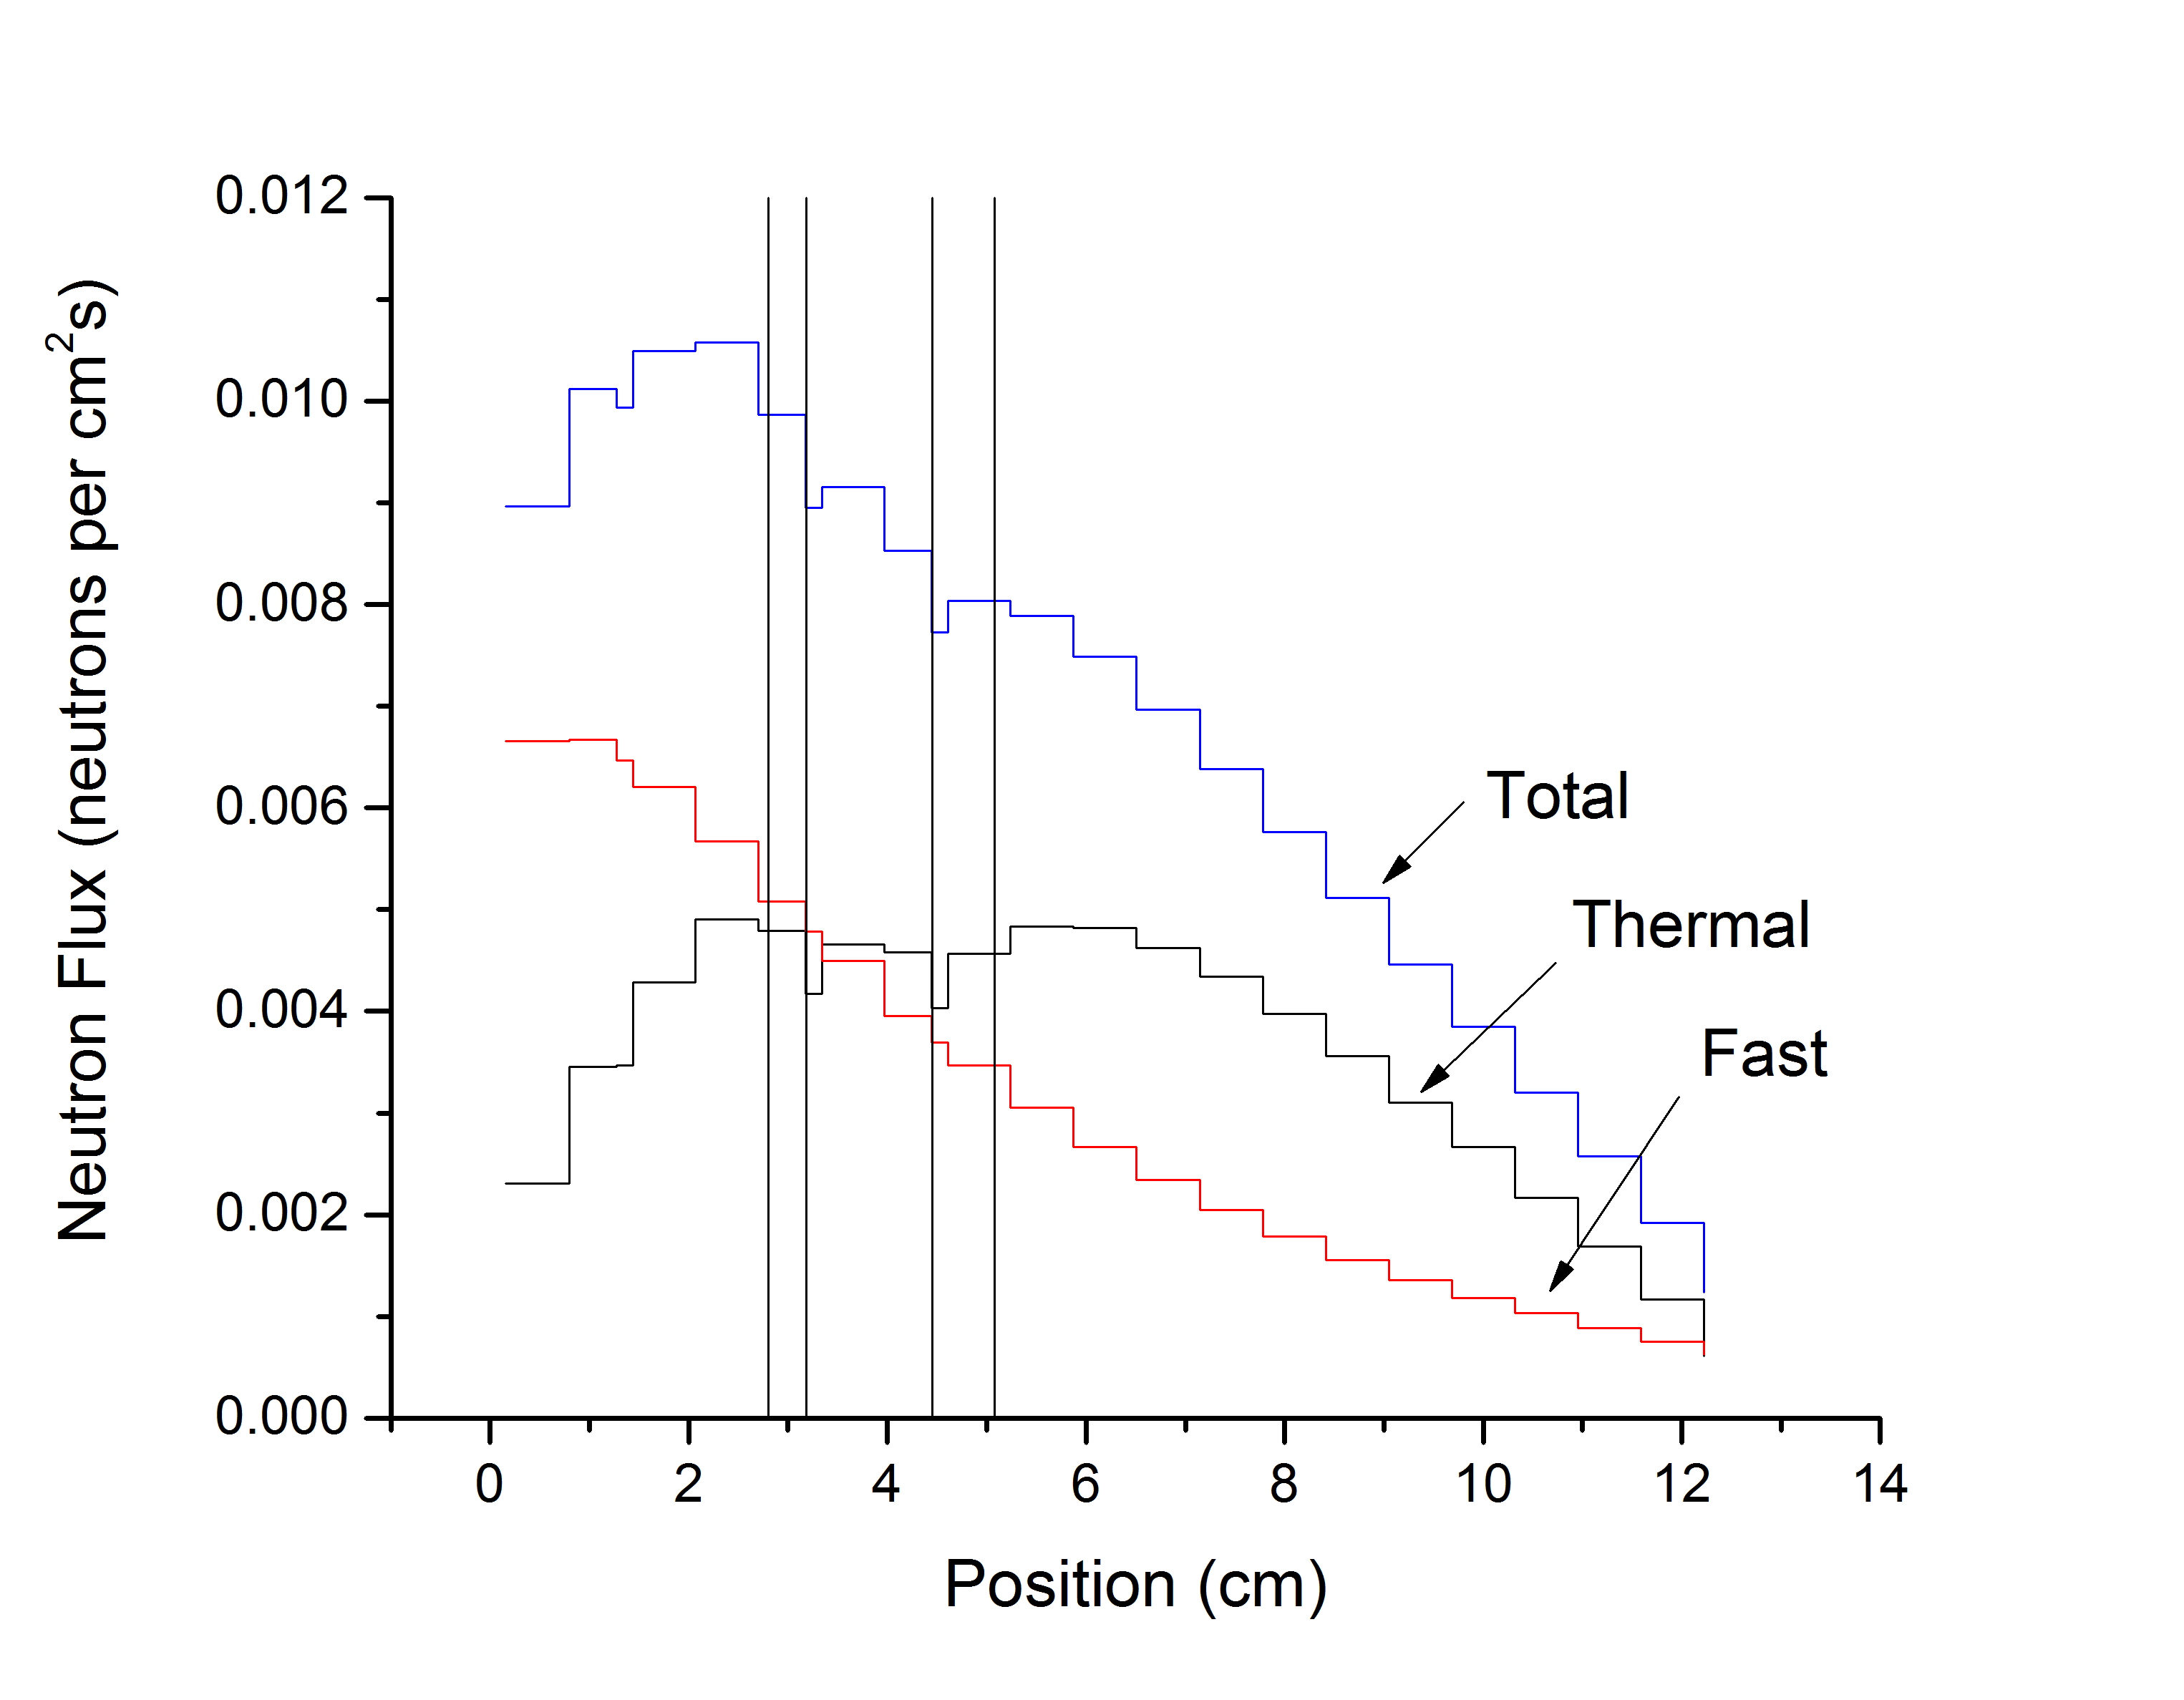
\includegraphics[width=\textwidth]{20Length25cpsMinFluxProfiles}
	\caption[Neutron Flux Profile for an Optimal 20 Length Genome, miniumn 2.5 interactions per second]{Neutron flux profile for a 20 length genome with an interaction rate of 3.82 interactions per neutron. The vertical lines represent detector slices.}
	\label{fig:20Length25MinFluxProfile}
\end{figure}
\begin{figure}
	\centering
	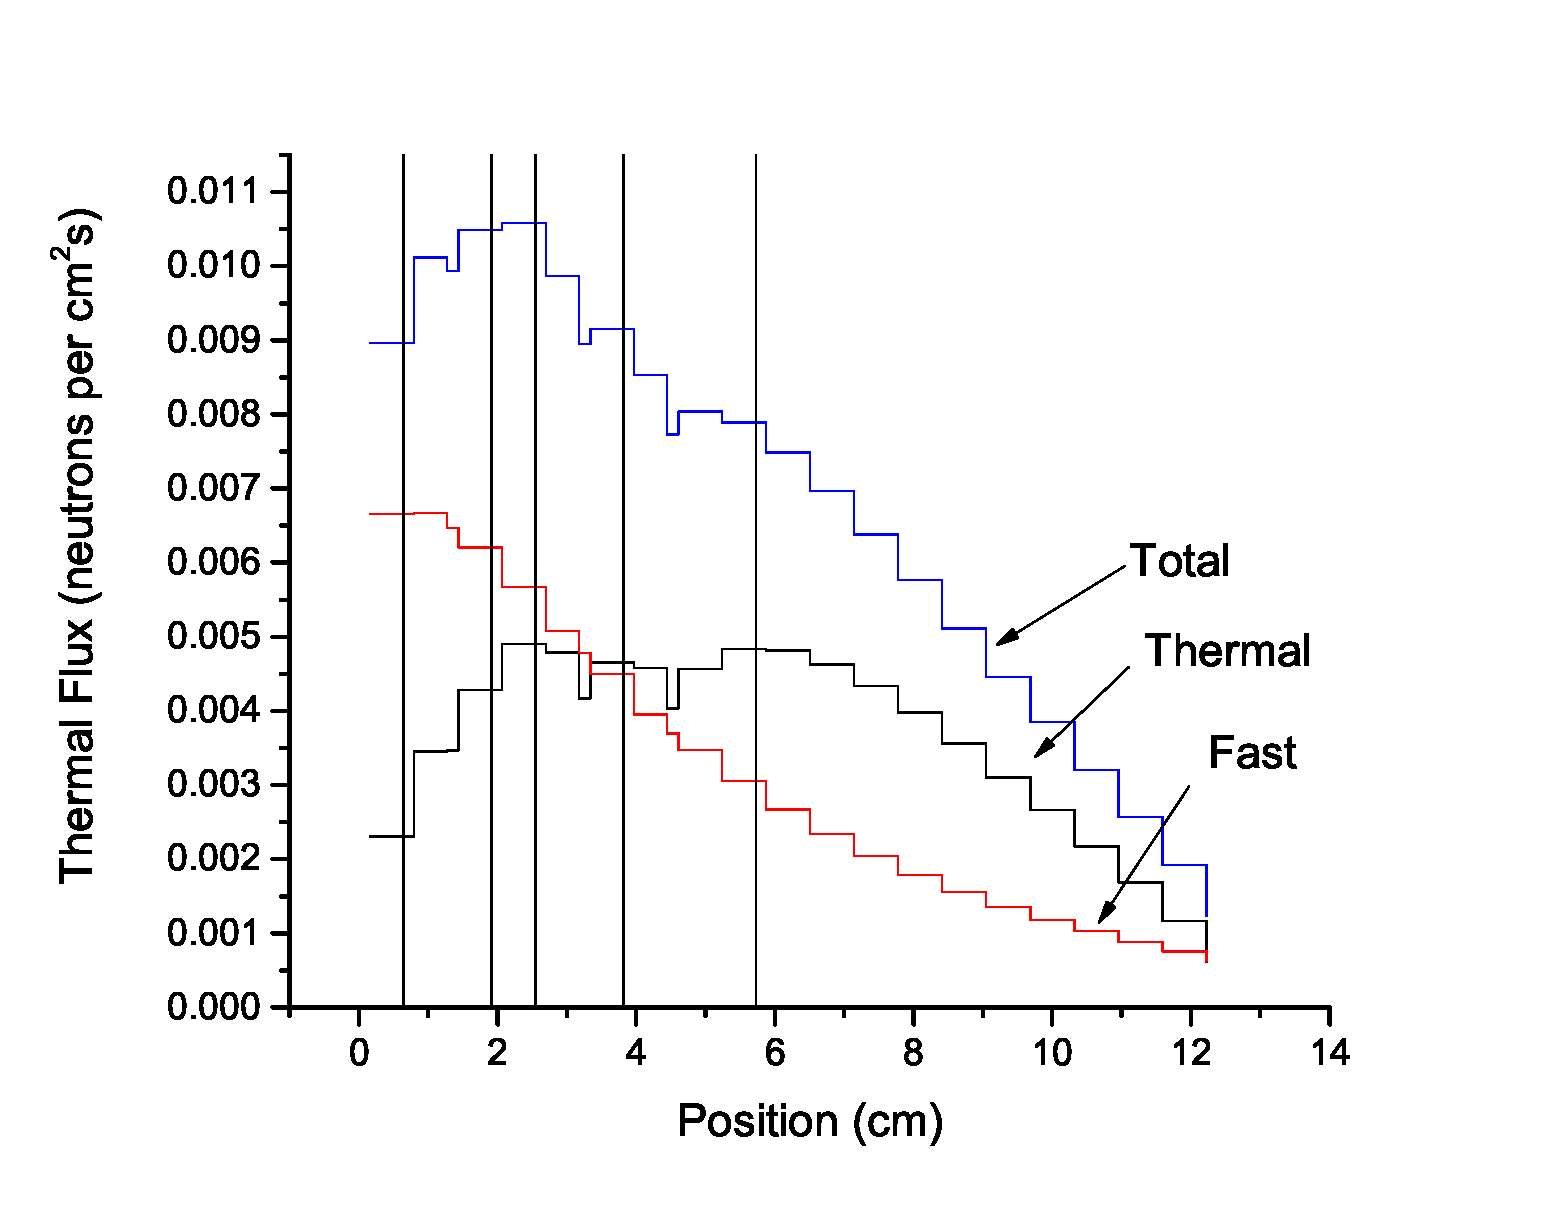
\includegraphics[width=\textwidth]{20Length5cpsMinFluxProfiles}
	\caption[Neutron Flux Profile for an Optimal 20 Length Genome, miniumn 5 interactions per second]{Neutron flux profile for a 20 length genome with an interaction rate of 5.31 interactions per neutron. The vertical lines represent detector slices.}
	\label{fig:20Length5MinFluxProfile}
\end{figure}
A physical basis of the optimal solution found by the genetic algorithm can be found by observing the form of the optimal solutions.
These solutions involve an initial moderator layer in order to ensure that all of the neutrons are thermalized to (increasing the thermal fraction by \textbf{SOME PERCENT}).
After this moderator layer a film layer is placed to utilize this neutron spectra; however not all of the thermal neutrons are captured (as the mean free path of a neutron in polyethylene is about \SI{0.37}{\cm} and thus some pass through the material) and another absorber layer is needed to capture those neutrons.  
The neutron flux is then moderated again, and additional layers of detectors are needed to capture this neutron cross section.
However, it is desirably to have a large neutron reflector in the portal monitor to reflect neutrons back into the detector slices. 
Theoretically this reflector should be as large as possible, but the limited space of the RPM provides a constraint.
A parameter study with a single detector slice between a moderator and reflector constrained by the radiation portal monitor design showed that it is desirable to have around \textbf{So much} moderator leaving the majority of the RPM to be left for the reflector.
Thus it is demonstrated that a large reflector is desired.

